% Klassendeklaration
\documentclass[
		fontsize=12pt,		% Schriftgröße 12pt
		toc=listof,		% Schreibt Tabellen/Abbildungs-Verzeichnisse auch mit ins Inhaltsverzeichnis
		%toc=bib,		% Literaturverzeichnis im Inhaltsverzeichnis aufführen
		%bibliography=openstyle	% Literaturverzeichnis etwas auflockern
		headsepline,		% Linie unter Kolumnentitel
		twoside=false,		% Layout für einseitigen Druck
		BCOR=12mm,		% Bindekorrektur: bei Buch normalerweise 12mm
		DIV=14,			% DIV-Wert fuer die Erstellung des Satzspiegels, siehe scrguide
		parskip=false,		% Absatzeinzug (Standard), half: kein Einzug, Halber Zeilenabstand, ...
		captions=tableheading,	% korrekte Abstände bei Tabellenüberschriften
		draft=false,		% true: Kennzeichnung von Absätzen, die manuell bearbeitet werden müssen, false: aus
		paper=A4,		% A4 Seite
		pagesize=automedia,	% Setzen der korrektern Papiergröße für Ausgabemedien
		numbers=noendperiod	% Auch wenn \appendix genutzt wird, keine Punkte hinter der Nummerierung (Regel im Duden sieht allerdings Punkt vor)
	]{scrbook}			% aus Komascript für Bücher
%%%%%%%%%%%%%%%%%%%%%%%%%%%%%%%%%%%%%%%%%%%%%%%%%%%%%%%%%%%%%%%%%%%%%%%%%%%%%%%%



% Pakete
\usepackage{cmap}		% to make the PDF files "searchable and copyable" in pdf viewer
\usepackage[ngerman]{babel}	% deutschsprachig
\usepackage[utf8]{inputenc}	% utf8 encoding
\usepackage[T1]{fontenc}	% Schriftkodierung
\usepackage{lmodern}		% skalierbare Schriftfamilie "Latin Modern" (default: bitmapped "Computer Modern")
\usepackage{graphicx}		% Einbinden von Grafiken
\usepackage{booktabs}		% weitere Linien zur Strukturierung von Tabellen (\toprule, ...)
\usepackage{multirow}		% mehrere Zeilen in einer Tabelle zusammenfassen
\usepackage{ltxtable}		% longtable und tabularx vereint in einer Tabelle, lädt automatisch beide Pakete
\usepackage{rotating}		% Text drehen
\usepackage{amsmath}		% Matheumgebung
\usepackage{amssymb}		% Zusatzsymbole zB Square Vartriangle etc
\usepackage{moreverb}		% erweiterte verbatim Umgebung
\usepackage{listings}		% Listings -> Quellcodedarstellung für viele verschiedene Sprachen
\usepackage{subfigure}		% Unterbilder
\usepackage{xcolor}		% Farbdefinitionen möglich
\usepackage{pdfpages}		% Einbinden von PDF Seiten aus PDF Dokument
\usepackage{nicefrac}		% Darstellung eines Bruchs im Fließtext; Aussehen zB 1/4
\usepackage{acronym}		% Abkürzungsverzeichnis --> nur verwendete Abkürzungen listen [printonlyused]
%\usepackage{bibgerm}		% deutsches Literaturverzeichnis
\usepackage{caption}		% viele caption Formatierungsmöglichkeiten
\usepackage{setspace}		% Zeilenabstand festlegen
\usepackage{microtype}		% Verbessert Textsatz
\usepackage{fixltx2e}		% Verbessert einige Kernkompetenzen von LaTeX2e
\usepackage{ellipsis}		% Korrigiert den Weißraum um Auslassungspunkte
\usepackage{units}		% Einheiten komfortabel darstellen \unit[Zahlenwert]{Einheit}
\usepackage{textcomp}		% einige Text-Mode Mathe Symbole, wie zB Mal-Zeichen x (siehe The Comprehensive LaTeX Symbol List)
\usepackage{gensymb}		% celsius, micro, ohm, perthousand, degree in Mathe und Textmodus
%%%%%%%%%%%%%%%%%%%%%%%%%%%%%%%%%%%%%%%%%%%%%%%%%%%%%%%%%%%%%%%%%%%%%%%%%%%%%%%%

% Einbindung von allen Grafikformaten möglich
\usepackage{pst-pdf} % pstricks und ps grafiken in pdflatex
\usepackage{pst-all}
\usepackage{pstricks-add}
%%%%%%%%%%%%%%%%%%%%%%%%%%%%%%%%%%%%%%%%%%%%%%%%%%%%%%%%%%%%%%%%%%%%%%%%%%%%%%%%


% für Fließumgebungen
% Platzierung H zwingt LaTeX Fließumgebungen genau an diese Stelle zu setzen
\usepackage{float}
\usepackage{wrapfig}
%%%%%%%%%%%%%%%%%%%%%%%%%%%%%%%%%%%%%%%%%%%%%%%%%%%%%%%%%%%%%%%%%%%%%%%%%%%%%%%%


% Kopf- und Fußzeilen
\usepackage[headsepline]{scrpage2}	% Paket, Linie unter Kopfangabe
\clearscrheadfoot			% löscht alle bisherigen Kopf- und Fußzeilen
\pagestyle{scrheadings}			% selbstgebastelte Kopf-/Fußzeilen
\automark{chapter}			% \automark[<rechte seite>]{<linke seite>}
\chead[Multicast Test Tool - Moduldokumentation Sender/Receiver - SPAM Software Programming And More]{Multicast Test Tool - Moduldokumentation Sender/Receiver - SPAM Software Programming And More} \cfoot[-\,\pagemark\,-]{-\,\pagemark\,-}% setzt Fußzeile [] -> chapterseiten; {} -> alle anderen Seiten
%%%%%%%%%%%%%%%%%%%%%%%%%%%%%%%%%%%%%%%%%%%%%%%%%%%%%%%%%%%%%%%%%%%%%%%%%%%%%%%%



% Schusterjungen und Hurenkinder vermeiden
\clubpenalty = 10000
\widowpenalty = 10000
\displaywidowpenalty = 10000
%%%%%%%%%%%%%%%%%%%%%%%%%%%%%%%%%%%%%%%%%%%%%%%%%%%%%%%%%%%%%%%%%%%%%%%%%%%%%%%%



% Farbdefinitionen
\definecolor{fill}{rgb}{1,1,0.73}
%%%%%%%%%%%%%%%%%%%%%%%%%%%%%%%%%%%%%%%%%%%%%%%%%%%%%%%%%%%%%%%%%%%%%%%%%%%%%%%%




% Workaround eines Bugs des wrapfig Paketes
% Entfernen wenn neue Version den Pakets verfügbar ist
% wenn ein umflossenes Bild nicht vollständig umflossen wird
% muss der Absatz geschlossen werden: dazu dann den Befehl
% \wrapfill hinter dem Absatz notieren
\usepackage{blindtext,wrapfig}
\makeatletter
\newcommand\wrapfill{\par
    \ifx\parshape\WF@fudgeparshape
    \nobreak
    \vskip-\baselineskip
    \vskip\c@WF@wrappedlines\baselineskip
    \allowbreak
    \WFclear
    \fi
}
\makeatother
%%%%%%%%%%%%%%%%%%%%%%%%%%%%%%%%%%%%%%%%%%%%%%%



% interne und externe Links werden als Hyperlinks übersetzt
% viele andere Optionen für pdf viewer möglich
% pdf metadaten
\usepackage{hyperref}
\hypersetup{pdftitle={Moduldokumentation Sender/Receiver},
	pdfauthor={Team 1},
	pdfsubject={Moduldokumentation Sender/Receiver},
	pdfcreator={LaTeX (TexLive 2008)},
	pdfproducer={LaTeX (TexLive 2008)},
	pdfkeywords={},
	colorlinks=true,
	urlcolor=black,
	linkcolor=black,
	citecolor=black,
	unicode=true
}
%%%%%%%%%%%%%%%%%%%%%%%%%%%%%%%%%%%%%%%%%%%%%%%%%%%%%%%%%%%%%%%%%%%%%%%%%%%%%%%%


% caption setup
% hang: bereich unter dem bezeichner bleibt frei;
% figurename: Bezeichner umdefinieren;
% margin: Einzug links und rechts
\captionsetup{format=hang,margin=30pt}
\captionsetup[lstlisting]{skip=13pt}
%%%%%%%%%%%%%%%%%%%%%%%%%%%%%%%%%%%%%%%%%%%%%%%%%%%%%%%%%%%%%%%%%%%%%%%%%%%%%%%%



%% Listings-Formatierung
\lstset{%
	language=Java, %
	basicstyle=\tiny,%\scriptsize,
	frame=trbl,%
	numbers=left,%
	breaklines=true,
	prebreak=\mbox{$\hookleftarrow$},
	postbreak=\mbox{$\longrightarrow$},
	breakatwhitespace=true,
	captionpos=t,%
	showstringspaces=false,
	numberstyle=\tiny,%
	commentstyle=\color{red},%
	keywordstyle=\bfseries\color{blue},%
	backgroundcolor=\color{fill},%
	rulecolor=\color{gray}%
}
%%%%%%%%%%%%%%%%%%%%%%%%%%%%%%%%%%%%%%%%%%%%%%%%%%%%%%%%%%%%%%%%%%%%%%%%%%%%%%%%

\setcounter{secnumdepth}{2}
\setcounter{tocdepth}{2}

% Tabellen
% neuer Spaltentyp C --> zentrierte X Spalten
\newcolumntype{C}{>{\centering\arraybackslash}X}
% Größere Höhe von Tabellenzellen
\renewcommand{\arraystretch}{1.3}
%%%%%%%%%%%%%%%%%%%%%%%%%%%%%%%%%%%%%%%%%%%%%%%%%%%%%%%%%%%%%%%%%%%%%%%%%%%%%%%%



% chapterüberschriften ohne Abstand zum Kopf festlegen
% \renewcommand*{\chapterheadstartvskip}{\vspace*{-\topskip}}
%%%%%%%%%%%%%%%%%%%%%%%%%%%%%%%%%%%%%%%%%%%%%%%%%%%%%%%%%%%%%%%%%%%%%%%%%%%%%%%%



% 1,5-Zeilenabstand (Paket setspace erforderlich)
\onehalfspacing
% Neuberechnung des Satzspiegels für neuen Zeilenabstand (DIV Angabe aus der
% Klassendeklartion übernommen)
\KOMAoptions{DIV=last}
%%%%%%%%%%%%%%%%%%%%%%%%%%%%%%%%%%%%%%%%%%%%%%%%%%%%%%%%%%%%%%%%%%%%%%%%%%%%%%%%



% Befehle für Hoch und Tiefstellen innerhalb eines Textes
\newcommand{\up}[2]{#1\textsuperscript{#2}}
\newcommand{\down}[2]{#1\textsubscript{#2}}
%%%%%%%%%%%%%%%%%%%%%%%%%%%%%%%%%%%%%%%%%%%%%%%%%%%%%%%%%%%%%%%%%%%%%%%%%%%%%%%%



% Beginn des Dokuments
\begin{document}

	%Vorspann
	\frontmatter

	% große römische Ziffern für die Seitennummern im Vorspann (Standard sind kleine römische Ziffern)
	\pagenumbering{Roman}

	% Includes Vorspann
	% Titelseite
	%%%%%%%%%%%%%%%%%%%%%%%%%%%%%%%%%%%%%%%%%%%%%%%%%%%%%%%%%%%%%%
% \titlehead	Kopfzeile der Titelseite
% \subject	Thema des Dokumentes
% \title	Titel des Dokumentes
% \subtitle	Untertitel
% \author	Autor des Dokumentes
% \date	Datum der Veröffentlichung
% \dedication	Widmung ;-)
% \publishers	Herausgeber
% \thanks	Fußnote
% \begin{abstract}
%   ...
% \end{abstract}

\newcommand{\mytitle}{}
\newcommand{\setmytitle}[1]{\renewcommand{\mytitle}{#1}}

\newcommand{\myauthor}{}
\newcommand{\setmyauthor}[1]{\renewcommand{\myauthor}{#1}}

\newcommand{\mysubject}{}
\newcommand{\setmysubject}[1]{\renewcommand{\mysubject}{#1}}

\setmytitle{"`Multicast Test Tool"'}
\setmyauthor{Tobias Stöckel, Tobias Schoknecht}
\setmysubject{Moduldokumentation GUI-Design}

\titlehead{%
	\fontsize{14pt}{12} \selectfont%
	\textbf{Fakultät:} \\%
	\\%
	
\includegraphics[width=5cm]{images/dhbw.jpg}

}

\title{}
\subject{\vspace{0.1cm}%
	\mysubject \\
	\vspace{0.5cm}%
	\mytitle%
	\vspace{-1.5cm}%
}
\author{%
	{
	\renewcommand{\arraystretch}{1}
	\fontsize{12pt}{12} \selectfont%
	\begin{tabular}{lcl}%
		Vorgelegt von & : & Team 1 \\%
		Verantwortlicher & : & Tobias Stöckel \\%
		Priorität aus Auftraggebersicht & : & mittel\\
		Priorität aus Auftragnehmersicht & : & hoch\\
		Stabilität & : & fest\\
		Kritikalität & : & niedrig\\
		Entwicklungsrisiko & : & niedrig\\
		Kategorie & : & Internes Dokument\\
		Version & : & 1.0\\
	 \end{tabular}%
	}
}
\date{

\includegraphics[height=3cm]{images/Logo.jpg}\\
16.05.2011
}

%%%%%%%%%%%%%%%%%%%%%%%%%%%%%%%%%%%%%%%%%%%%%%%%%%%%%%%%%%%%%%%%
\maketitle
	% Includes Verantwortliche
	% Titelseite
	%\chapter*{Projektteam}
\textbf{Produkt Manager}\\
Tobias St"ockel\\
\newline
\textbf{Projekt Leiter}\\
David Hildenbrand\\
\newline
\textbf{Leitende Ingenieure}\\
Jeffrey Jedele\\
Konstantin Weitz\\
\newline
\textbf{Technische Dokumentation}\\
Tobias Schoknecht\\
\newline\textbf{Systemtest}\\
Ramin Safarpour\\
\newline
	%%%%%%%%%%%%%%%%%%%%%%%%%%%%%%%%%%%%%%%%%%%%%%%%%%%%%%%%%%%%%%%%%%%%%%%%%%%%%%%%
	% offizielle Aufgabenstellung
%	\include{./chapter/aufgabenstellung}
	%%%%%%%%%%%%%%%%%%%%%%%%%%%%%%%%%%%%%%%%%%%%%%%%%%%%%%%%%%%%%%%%%%%%%%%%%%%%%%%%
	% Selbstständigkeitserklärung
	%\include{./chapter/declaration_of_primary_authorship}
	%%%%%%%%%%%%%%%%%%%%%%%%%%%%%%%%%%%%%%%%%%%%%%%%%%%%%%%%%%%%%%%%%%%%%%%%%%%%%%%%
	% Inhaltsverzeichnis
	\tableofcontents
	%%%%%%%%%%%%%%%%%%%%%%%%%%%%%%%%%%%%%%%%%%%%%%%%%%%%%%%%%%%%%%%%%%%%%%%%%%%%%%%%
	% Abbildungsverzeichnis
	\listoffigures
	%%%%%%%%%%%%%%%%%%%%%%%%%%%%%%%%%%%%%%%%%%%%%%%%%%%%%%%%%%%%%%%%%%%%%%%%%%%%%%%%
	% Tabellenverzeichnis
	\listoftables
	%%%%%%%%%%%%%%%%%%%%%%%%%%%%%%%%%%%%%%%%%%%%%%%%%%%%%%%%%%%%%%%%%%%%%%%%%%%%%%%%
	% Listings-Verzeichnis
%	\renewcommand{\lstlistlistingname}{Quelltexte}
%	\lstlistoflistings
	%%%%%%%%%%%%%%%%%%%%%%%%%%%%%%%%%%%%%%%%%%%%%%%%%%%%%%%%%%%%%%%%%%%%%%%%%%%%%%%%
	% Abkürzungsverzeichnis/Formelzeichen
	%\addcontentsline{toc}{chapter}{Abkürzungsverzeichnis}
\chapter*{Abkürzungsverzeichnis}

    \begin{description}
        \item[PPS] Packets Per Second. (Multicast-) Pakete pro Sekunde. Einheit
        für Datensende- und empfangsrate.
    \end{description}
	%%%%%%%%%%%%%%%%%%%%%%%%%%%%%%%%%%%%%%%%%%%%%%%%%%%%%%%%%%%%%%%%%%%%%%%%%%%%%%%%
	%%%%%%%%%%%%%%%%%%%%%%%%%%%%%%%%%%%%%%%%%%%%%%%%%%%%%%%%%%%%%%%%%%%%%%%%%%%%%%%%

	% Hauptteil
	\mainmatter

	
\chapter{Scope}
Die Moduldokumentation beschreibt die Architektur, die Schnittstellen 
und die Hauptmerkmale des Moduls. Außerdem werden die Modul bzw. Komponententests 
einschließlich der Ergebnisse beschrieben und dokumentiert. 
Die MOD dient bei Bedarf auch als Programmier- oder Integrationshandbuch für das 
Modul. Wenn bestimmte Risiken direkt mit der Verwendung des Moduls verknüpft sind,
so sind sie in diesem Dokument zu benennen und zu kommentieren.

\chapter{Definitionen}

\section{Abkürzungen}

    \begin{description}
    \item[GUI] Graphical User Interface. Grafische Benutzeroberfläche
    \item[IDE] Integrated Development Environment. Integrierte
    Entwicklungsumgebung. Ein Softwarepaket, dass Prozesse der
    Softwareentwicklung unterstützt.
    \end{description}

%\section{Definitionen}
%Wichtige Begriffe und Worte

%\section{Terminologien}
%Besondere Begrifflichkeiten und deren Verwendung.
%Festgelegte Terminologien und Regeln für Schreibweise z.B. Notationsegeln für CLI Kommandos


\chapter{Analyse}
Das Gesamtsystem wird zur besseren Verständlichkeit und zur Vermeidung von Ab-
hängigkeiten in logische Komponenten unterteilt.
Auf höchster Abstraktionsebene ist das strukturgebende Element der Anwendung ein
Model-View-Controller Pattern. Dieses Pattern gliedert die Applikation in drei Unter-
module, das Model, die View und den Controller. Die Entscheidung dieses Pattern zu
benutzen fiel auf Grund der vielen architektonischen Vorteile. So herrscht zwischen
den einzelnen Komponenten eine strenge Hierarchie. Das Model weiß von keinem Con-
troller und der Controller kennt keine View. Durch diese Trennung besteht eine sehr
schwache Kopplung zwischen den einzelnen Komponenten. Zudem lässt sich die View
sehr flexibel gestalten und es können sogar mehrere Views zur gleichen Zeit aktiv sein,
ohne sich gegenseitig zu stören. Diese Flexibilität der View ist ausschlaggebend für die
Anpassungsfähigkeit der Applikation an ein sich änderndes Umfeld. Die tatsächliche
Lösung des Problems behält nämlich meistens über einen relativ langen Zeitraum seine
Berechtigung, während sich die Anforderungen an die Visualisierung und Bedienung
der eigentlichen Programmlogik viel schneller ändern. Aber der wohl wichtigste Grund
ist die Bewährtheit des Patterns. So wird er von den meisten modernen Applikationen
umgesetzt und findet sich auch in jeder modernen GUI Library wieder. Der einzige
Nachteil des Patterns sind Performance Einbusen, wie sie bei den meisten Ansätzen der
architektonischen Strukturierung anfallen.

%Dieses Kapitel muss alles beinhalten, was noch nicht in anderen Dokumenten enthalten ist.

\section{Voruntersuchungen}

    Der endgültigen GUI-Implementierung gingen zahlreiche Voruntersuchungen,
    Prototypen und die Evaluation verschiedener Vorgehensweisen voraus.

    \subsection{Java Swing-Toolkit}
    
        Ein großer Teil der Voruntersuchungen bezieht sich auf die Eigenheiten
        und Best-Practices im Umgang mit dem Swing-Toolkit. Diverse Prototypen
        wurden entwickelt, um das Verhalten von Dialogen und Tabellen zu
        evaluieren.
        
        Auch die Umsetzung der Swing-Threading-Policy erforderte
        gründliche Voruntersuchungen. Diese Policy erfordert, dass außer dem
        Swing-Worker-Thread kein weiterer Thread auf die Elemente der grafischen
        Oberfläche zugreift. Dies stellte eine besondere Herausforderung dar, da
        das Multicast Test Tool stark auf Multi-Threading basiert. Jeder Sender
        und Empfänger läuft in einem eigenen Thread und schickt ständig
        Aktualisierungen an die View.
        
    \subsection{Netbeans GUI-Designer}
    
        Für die Erzeugung des statischen GUI-Codes fiel die Wahl auf den
        GUI-Designer der Netbeans-IDE. Dessen Fähigkeiten, gerade auch in Bezug
        auf Internationalisierung wurden im Vorfeld gründlich untersucht. So
        zeigte sich, dass der GUI-Designer trotz gewisser Einschränkungen die
        für das Projekt benötigte Mächtigkeit und Flexibilität mitbringt. Die
        Einschränkungen bestehen hauptsächlich darin, dass der generierte Code
        zum Teil nicht von Hand nachbearbeitet werden darf, um die
        Kompatibilität mit dem GUI-Designer zu gewährleisten.
        
        Als einziger großer Nachteil hat sich erwiesen, dass der Designer
        zusätzlich zum Code separate XML-Dateien erzeugt, in denen die Struktur
        einer GUI-Komponente festgehalten ist. Diese Dateien sind von Hand kaum
        wartbar, was zum Beispiel beim Zusammenführen von Änderungen mithilfe
        der Versionsverwaltung zu Problemen führte.
        
        Nichtsdestotrotz ist der Code aller GUI-Komponenten zum Zeitpunkt der
        Übergabe noch immer mit dem GUI-Designer kompatibel, was eine
        Weiterentwicklung deutlich vereinfacht.
        
    \subsection{Java Application Framework}
    
        Zu Beginn wurden kurz die Möglichkeiten des Java Application Framework
        evaluiert. Dieses Framework vereinheitlicht die Zusammenarbeit von View
        und Controller, sowie Standard-Aufgaben der GUI-Verwaltung. Zu diesen
        Standardaufgaben gehören zum Beispiel die Internationalisierung, das
        zentrale Verwalten von Java-Actions, sowie das Persistieren des
        GUI-Zustandes (Fenstepositionen für den nächsten Start merken, etc.).
        
        Da die Verwendung dieses Frameworks allerdings erhebliche Änderungen an
        der Architektur des Controllers nach sich gezogen hätte, wurde auf sie
        verzichtet.
        
    \subsection{Internationalisierung}
    
        Zwecks Internationalisierung wird auf den
        Java-ResourceBundle-Mechanismus zurückgegriffen, dessen Arbeitsweise
        zunächst evaluiert werden musste.
        
    \subsection{Layout-Manager}
    
        Selbst bei Verwendung eines GUI-Designers, ist es unerlässlich sich mit
        den Swing-Layout-Managern auseinanderzusetzen. Gerade im Hauptfenster
        wurden die Layout-Manager sämtlich von Hand konfiguriert.
        
        Die exakte Arbeitsweise der Manager und deren korrekte Anwendung wurde
        in diversen Prototypen ausgiebig getestet.
        
     \subsection{Tabellen}
     
        Kernstück und größte Herausforderung der grafischen Oberfläche sind die
        beiden Tabellen, die Sender und Empfänger darstellen. Um sie in dem
        Umfang anzupassen, wie in diesem Projekt geschehen, wurde die
        Arbeitsweise der Swing-JTable, sowie deren Code in großem Maßstab
        untersucht.
        
        Die Entwicklung der darstellenden Tabellen, sowie der zugrundeliegenden
        TableModels, erforderte eine umfangreiche Analyse und zahlreiche
        Prototypen. Um eine korrekte Darstellung des Folding-Mechanismus der
        Empfängertabelle zu erreichen wurde die JTreeTable von Philip Milne
        ausgiebig analysiert und selbst wenn diese Funktionalität dann doch von
        Grund auf in Eigenentwicklung entstand, so sind doch viele Anregungen
        aus Milnes Artikel übernommen worden.
        
        In den Voruntersuchungen, wurde auch der Versuch analysiert, die
        Tabelle komplett neu und ohne Verwendung der vom Swing-Toolkit
        bereitgestellten JTable zu programmieren. Dieser Weg wurde aber aufgrund
        des großen Aufwands und der festgestellten großen Ähnlichkeit zur
        JTable aufgegeben.

\section{Systemanalyse}

    \subsection{Rahmenbedingungen}
    
        Die GUI-Logik ist das Bindeglied zwischen dem Controller des Multicast
        Test Tools und dem Design der grafischen Oberfläche. Das Modul ist per
        Observer-Pattern an den Controller und das Model angebunden.
        Manipulierenden Zugriff auf das Model erhält die GUI-Logik über den
        Controller. Für die Internationalisierung steht der systemweite
        ResourceBundle-Mechanismus zur Verfügung.
    
    \subsection{Problemstellung}
    
        Hauptaufgabe der GUI-Logik ist es, Ereignisse des Models für die
        darstellenden View-Komponenten aufzubereiten und weiterzureichen.
        
        Die Veranwortung der GUI-Logik besteht auch darin, die
        Swing-Threading-Policy zuverlässig umzusetzen. Wie in den Voruntersuchungen
        erwähnt, müssen dazu alle eingehenden Events, die aus unvorhersehbaren
        Model-Threads stammen können, mit besonderer Vorsicht gehandhabt werden.
        
        Als dritten Punkt, muss die GUI-Logik Nutzerinteraktion für die
        Applikation aufbereiten und über den Controller an das Model
        weiterreichen.
        
        Die Nutzeroberflächen und Ausgaben müssen international betextbar sein. Mit der
        Endversion der Software werden die Sprachen Deutsch und Englisch ausgeliefert. Weiter
        Sprachen müssen einfach mit Klartext-Dateien hinzugefügt werden können.
    
    \subsection{Abhängigkeiten}

        Die gesamte View ist funktional stark abhängig von Model und Controller
        der Anwendung. Immerhin müssen alle möglichen Model-Zustände von der
        View angemessen wiedergegeben werden, sowie der volle Funktionsumfang
        von Model und Controller über die Vew zugänglich sein.
        
        Auf der anderen Seite wurde peinlichst darauf geachtet, keine
        Abhängigkeiten des Models und des Controllers zur View einzuführen.
        Sowohl Model, als auch Controller kommunizieren ausschließlich über
        flexible Ereignis-Mechanismen mit der View. Aus diesem Grund ist die
        View auch in Zukunft eine Komponente, die ohne Probleme ausgetauscht und
        an sich gegebenfalls ändernde Anforderungen an die Ergonomie angepasst
        werden kann.

\chapter{Design}

    \section{Lösungen für Problembereich der Analyse}
    
        Um die Aufbereitung der Modeldaten für die GUI zu strukturieren,
        werden für komplexere Komponenten eigene "`Data Models"' eingeführt.
        Diese stellen eine Zwischenstufe in der Datenorganisation dar und können
        von darstellenden Komponenten direkt umgesetzt werden. Die GUI-Logik
        greift dann nur noch auf diese Data Models zu.
        
        Um die Swing-Threading-Policy korrekt umzusetzen, werden alle von Model
        und View ankommenden Ereignisse an zentraler Stelle vom GUI-Controller
        in den Swing-Worker-Thread und dessen Event-Queue eingereiht. Dadurch wird eine
        sequentielle und sichere Abarbeitung der Ereignisse gewährleistet, was
        für einen ständig konsistenten Zustand der grafischen Oberfläche
        unerlässlich ist.
        
        Alle Nutzerinteraktionen, die auf eine Manipulation des Models
        hinauslaufen, werden vom View-Controller gesammelt und an den Controller
        der Anwendung weitergereicht.
        
        In diesem Modul werden alle Internationalisierungsdetails hinter einem sehr
        einfachen Interface verborgen. Die Komponente kümmert sich um das laden der Sprach-
        dateien und übersetzt übergebene Template Strings in die gewählt Sprache und kümmert
        sich zudem um die Ersetzung von Platzhaltern in den Strings und die Übersetzung von
        Exceptions.
    
    \section{Systemarchitektur}
    
        Die grundsätzliche Architektur ist in drei Teilbereiche aufgegliedert:
        
        Eine zentrale Klasse dient als Schnittstelle zu Controller und Model.
        Sie reicht Ereignisse sowohl an den Controller, als auch an die
        restlichen Komponenten der GUI weiter. Außerdem steuert sie die korrekte
        Initialisierung und Beendigung der GUI. Diese Klasse fungiert also quasi
        als Controller für die View. Aus diesem Grund wird auf sie im Folgenden
        auch als "`View-Controller"' Bezug genommen.
        
        Das Hauptfenster und dessen Komponenten sind in ein eigenes Paket
        gekapselt. Es erhält Aktualisierungen vom View-Controller, steuert sein
        endgültiges optisches Verhalten aber selbst.
        
        Der dritte Teilbereich umfasst die Dialoge, die zur Benutzerinteraktion
        genutzt werden. Dazu gehören Dialoge zum Anlegen und Bearbeiten von
        Sendern und Empfängern, zum Anzeigen detaillierter Statistiken, zum
        Laden und Speichern von Konfigurationsdateien, sowie Fehlermeldungen.
        Die Dialoge werden entweder direkt aus dem Hauptfenster, als Reaktion
        auf Benutzeraktionen eingeblendet und ausgewertet, oder aber nach
        eingegangen Fehlerereignissen vom View-Controller erzeugt.
        
        Eine Übersicht über die wichtigsten Klassen des View-Moduls bietet
        Diagramm \ref{view_architecture}.
    
    \section{Schnittstellen}
    
        Mit dem View-Controller, bietet die View dem Rest der Anwendung eine
        zentrale Schnittstelle. Über ihn werden alle nötigen Informationen an
        die View weitergereicht. 
        
        Auch für die restlichen View-Komponenten ist der View-Controller die
        Schnittstelle zu Model und Controller der Anwendung.
        
        Insgesamt ist die View aus bereits genannten Gründen sehr stark an Model
        und Controller gekoppelt. Auch in sich besteht aufgrund der starken
        Abhängigkeit zwischen GUI-Logik und -Design eine starke Kohäsion.


    %Folgerungen aus der Analyse 
    %Lösungen für den Problembereich der Analyse 
    %Systemarchitektur 
    %Anwendung der Basiskonzepte des Softwareengineerings
    %Schnittstellen

\chapter{Implementierung}

    \section{View-Controller}
    
        Den View-Controller stellt die GraphicalView-Klasse dar. Sie ist der in
        der System Architecture Specification vorgesehene Einstiegspunkt zur
        grafischen Benutzeroberfläche.
        
        Die GraphicalView implementiert die benötigten Listener für die
        unterschiedlichen Ereignisse von Model und Controller. Sie ist außerdem für die korrekte
        Initialisierung des Hauptfensters und der Dialoge verantwortlich und
        muss dafür sorgen, sich bei allen notwendigen Ereignisquellen zu
        registrieren.
        
        Im laufe der Implementierung zeigte sich immer deutlicher der
        "`durchreichende"' Character dieser Klasse. Viele Ereignisse können erst
        in einer konkreten GUI-Komponente angemessen ausgewertet werden.
    
    \section{Hauptfenster}
    
        Vorweg ist zu bemerken, dass das Grundgerüst der Logik des Hauptfensters
        größtenteils vom Netbeans GUI-Designer vorgegeben wurde. Daher zum
        Beispiel die Entscheidung, ActionListener als anonyme Klassen zu
        realisieren, und alle ActionEvents in der Hauptfenster-Klasse selbst zu
        behandeln.
        
        Das Hauptfenster verwaltet seinen visuellen Zustand selbst. Dazu werden
        vom View-Controller aufbereitete Daten in ihre visuelle Entsprechung
        umgewandelt, was zum Beispiel die Anpassung eines Textfeldes, oder eine
        Farbänderung in einer GUI-Komponente zur Folge hat.
        
        Alle vom Benutzer ausgeführten Aktionen werden in dieser Klasse
        aufgefangen und entweder direkt in ihre visuelle Entsprechung umgesetzt,
        oder an den View-Controller weitergeleitet.
        
        Eine Ausnahme bildet hier das eventuelle Aufrufen eines Dialogs, was
        durch die Hauptfenster-Klasse direkt, ohne Umweg über den
        View-Controller, vorgenommen wird. Dies hat vor Allem den Grund, das ein
        Dialog im Swing-Toolkit stets eng an sein "`Parent"', in diesem Fall das
        Hauptfenster, gebunden ist. Ein Dialog kann also getrost als
        Teilkomponente des Hauptfensters betrachtet werden.
    
    \section{Dialoge}
    
        Die Dialoge sind in kleinerem Maßstab ähnlich wie das Hauptfenster
        angelegt. Sie verwalten den Zustand ihrer Komponenten selbst und reichen
        eventuelle Nutzeraktionen an ihren Aufrufer, bzw. in manchen Fällen
        direkt an das Model weiter.
        
        Die Dialoge für Statistik-Detailansichten stellen zusätzlich einen
        Mechanismus zur Verfügung, der es ermöglicht, die angezeigten Daten
        regelmäßig zu aktualisieren.
        
    \section{Codedokumentation}
    
        Der Code der GraphicalView und aller Subkomponenten wurde ausführlichst
        gemäß Javadoc-Konventionen dokumentiert.
%Vorgehen 
%Zwischenergebnisse 
%Anwendung der Basiskonzepte 
%Codedokumentation 

% \chapter{Komponententest}
% %Wie wird die Komponente getestet? 
% %Dokumentation von Vorgehen und Ergebnissen. Bei Bedarf entsprechend erweitern
% 
% Die korrekte Funktionsweise der GUI-Komponenten wurde im Rahmen der
%     Continouus Integration projektbegleitend von Hand getestet. Automatisierte
%     Testverfahren wurden zwar evaluiert, deren konsequenter Einsatz erwies sich
%     jedoch als nicht wirtschaftlich.
% 
% \section{Komponententestplan}
% 
% \begin{table}[h]
% \caption{Komponententestplan}
% \label{tab:ktp}
% \begin{center}
% \begin{tabular}{|p{2cm}|p{3cm}|p{9cm}|}
% \hline
% \textbf{Test Nr.} & \textbf{Feature ID} & \textbf{Test Spezifikation}\\
% \hline
%  & & \\
% \hline
%  & & \\
% \hline
%  & & \\
% \hline
%  & & \\
% \hline
% \end{tabular}
% \end{center}
% \end{table}
% 
% \section{Komponententestreport}
% 
% \begin{table}[h]
% \caption{Komponententestreport}
% \label{tab:ktr}
% \begin{center}
% \begin{tabular}{|p{2cm}|p{2cm}|p{6cm}|p{1.5cm}|p{1.5cm}|}
% \hline
% \textbf{Test Nr.} & \textbf{Pass/Fail} & \textbf{Test Ergebnis (wenn Fail)} & \textbf{Datum} & \textbf{Tester}\\
% \hline
%  & & & &\\
% \hline
%  & & & &\\
% \hline
%  & & & &\\
% \hline
%  & & & &\\
% \hline
% \end{tabular}
% \end{center}
% \end{table}

\chapter{Zusammenfassung}

\section{Beurteilung der Komponente}
%Hat die Komponente Schwächen und Stärken, 
%Besonderheiten?
%Übertragbarkeit der Komponente und Lösungen
%Was ist verbesserungswürdig?

    Eine Besonderheit und Herausforderung der GUI-Logik besteht in ihrer hohen
    Abhängigkeit sowohl von Model und Controller, als auch von den visuellen
    GUI-Komponenten. Zudem besteht bei GUI-Code stets die Gefahr, dass er sehr
    ausufernd und unübersichtlich wird. In diesem Fall wurde dieses Problem
    damit umgangen, dass für die Verwaltung des statischen GUI-Codes ein
    GUI-Designer zur Verwendung kam.
    
    Eine große Schwäche dieses Moduls sind die starken inneren Abhängigkeiten.
    Gezielte Änderungen an einzelnen Komponenten werden sich hier wohl sehr
    schwierig gestalten. Außerdem ist in diese Modul noch Redundanz bezüglich
    der Benutzeraktionen enthalten. Dieselbe Benutzeraktion (z.B. "`Anlegen
    eines Senders"') ist an allen Stellen, an denen sie in der GUI zugänglich
    ist, einzeln auscodiert, bzw. kompliziert umgeleitet. Ein Lösungsansatz
    hierfür findet sich im folgenden Abschnitt Ausblick für die
    Weiterentwicklung.
    
    Als positiv zu vermerken ist die elegant und effizient umgesetzte
    Internationalisierung der grafischen Oberfläche, die sogar ein Umschalten
    der Sprache im laufenden Betrieb ermöglicht. Auch die zentralisierte
    Verwaltung von Initialisierung und Model-Ereignissen durch den
    View-Controller hat sich als hilfreich erwiesen. Gerade die
    Swing-Threading-Policy konnte so zuverlässig umgesetzt werden. Eine weitere
    Stärke ist die Verwaltung der Daten komplexer View-Komponenten in eigenen
    Data Models. Sie tragen entscheidend zur konsistenz dieser Daten in der
    gesamten GUI bei.

\section{Ausblick für die Weiterentwicklung}
%Sind schon Dinge vorbereitet?
%Erweiterungsmöglichkeiten?

    Der nächste Schritt, um die Implementierung der GUI zu vereinheitlichen wäre
    die Umsetzung des Java-Action-Konzepts für Benutzeraktionen. Dieses Konzept
    würde GUI-Logik und visuelle Komponenten stärker von einenander Kapseln und
    den Code-Wiederverwendungsgrad innerhalb der Komponente erhöhen.
    
    Weiterhin müssten die Datenflüsse der View genau analysiert werden, um
    eventuelle Lecks, also direkte Zugriffe auf Model oder Controller aus
    internen GUI-Komponenten, aufzudecken und zu eliminieren. Dieser Schritt
    würde die Abhängigkeit der View von einer konkreten Model-Implementierung
    weiter verringern.

    Grundsätzlich ist aber die gesamte Architektur darauf ausgelegt, dass die
    gesamte View in Zukunft ohne Weiteres durch eine neue (bessere?)
    Implementierung ersetzt werden kann.

%\chapter{Referenzen und Standards}
	
	%%%%%%%%%%%%%%%%%%%%%%%%%%%%%%%%%%%%%%%%%%%%%%%%%%%%%%%%%%%%%%%%%%%%%%%%%%%%%%%%

	\begin{appendix}

	\chapter{Diagramme}

\begin{figure}[H]
\center
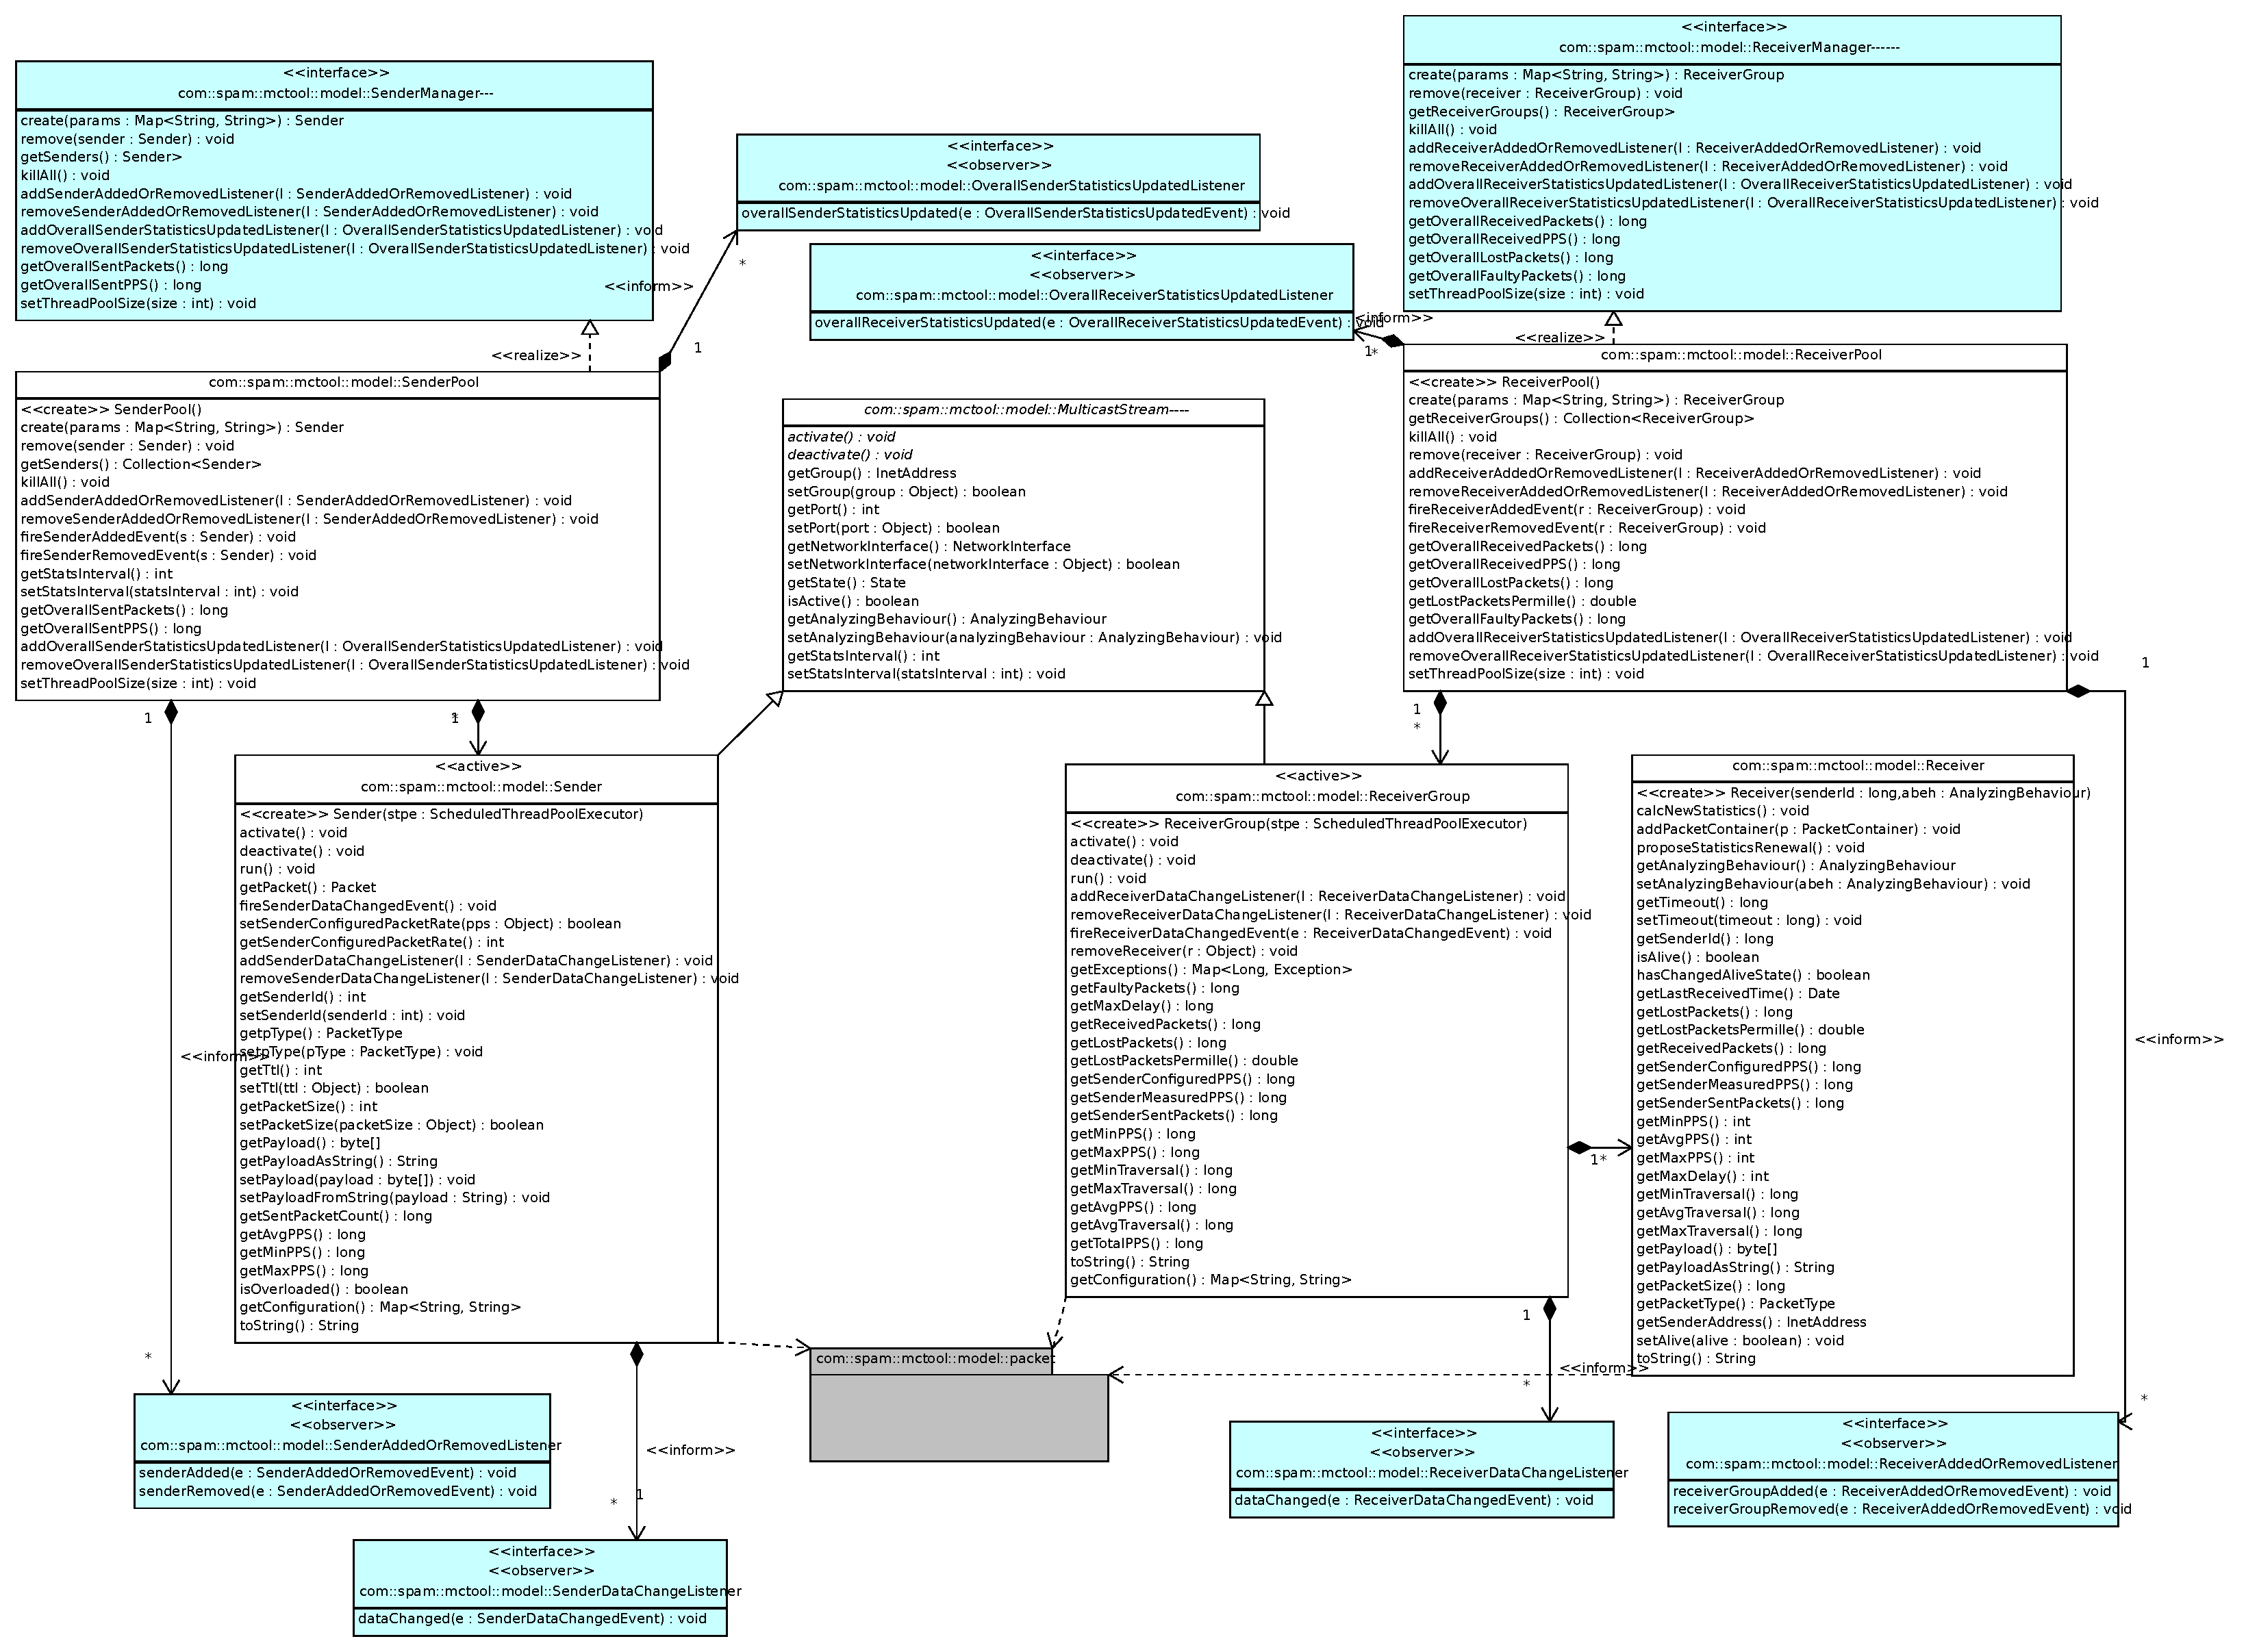
\includegraphics[width=19cm,angle=90]{images/model_detail.pdf}
\caption{Vollständige ESK}
\end{figure}	

	\chapter{Schnittstellendefinitionen}
Die ESK kommuniziert über mehrere Schnittstellen mit dem Rest des Systems.
Folgende UML Diagramme beschreiben die im Modell spezifizierten und verwendeten
Schnittstellen

\begin{figure}[H]
\center
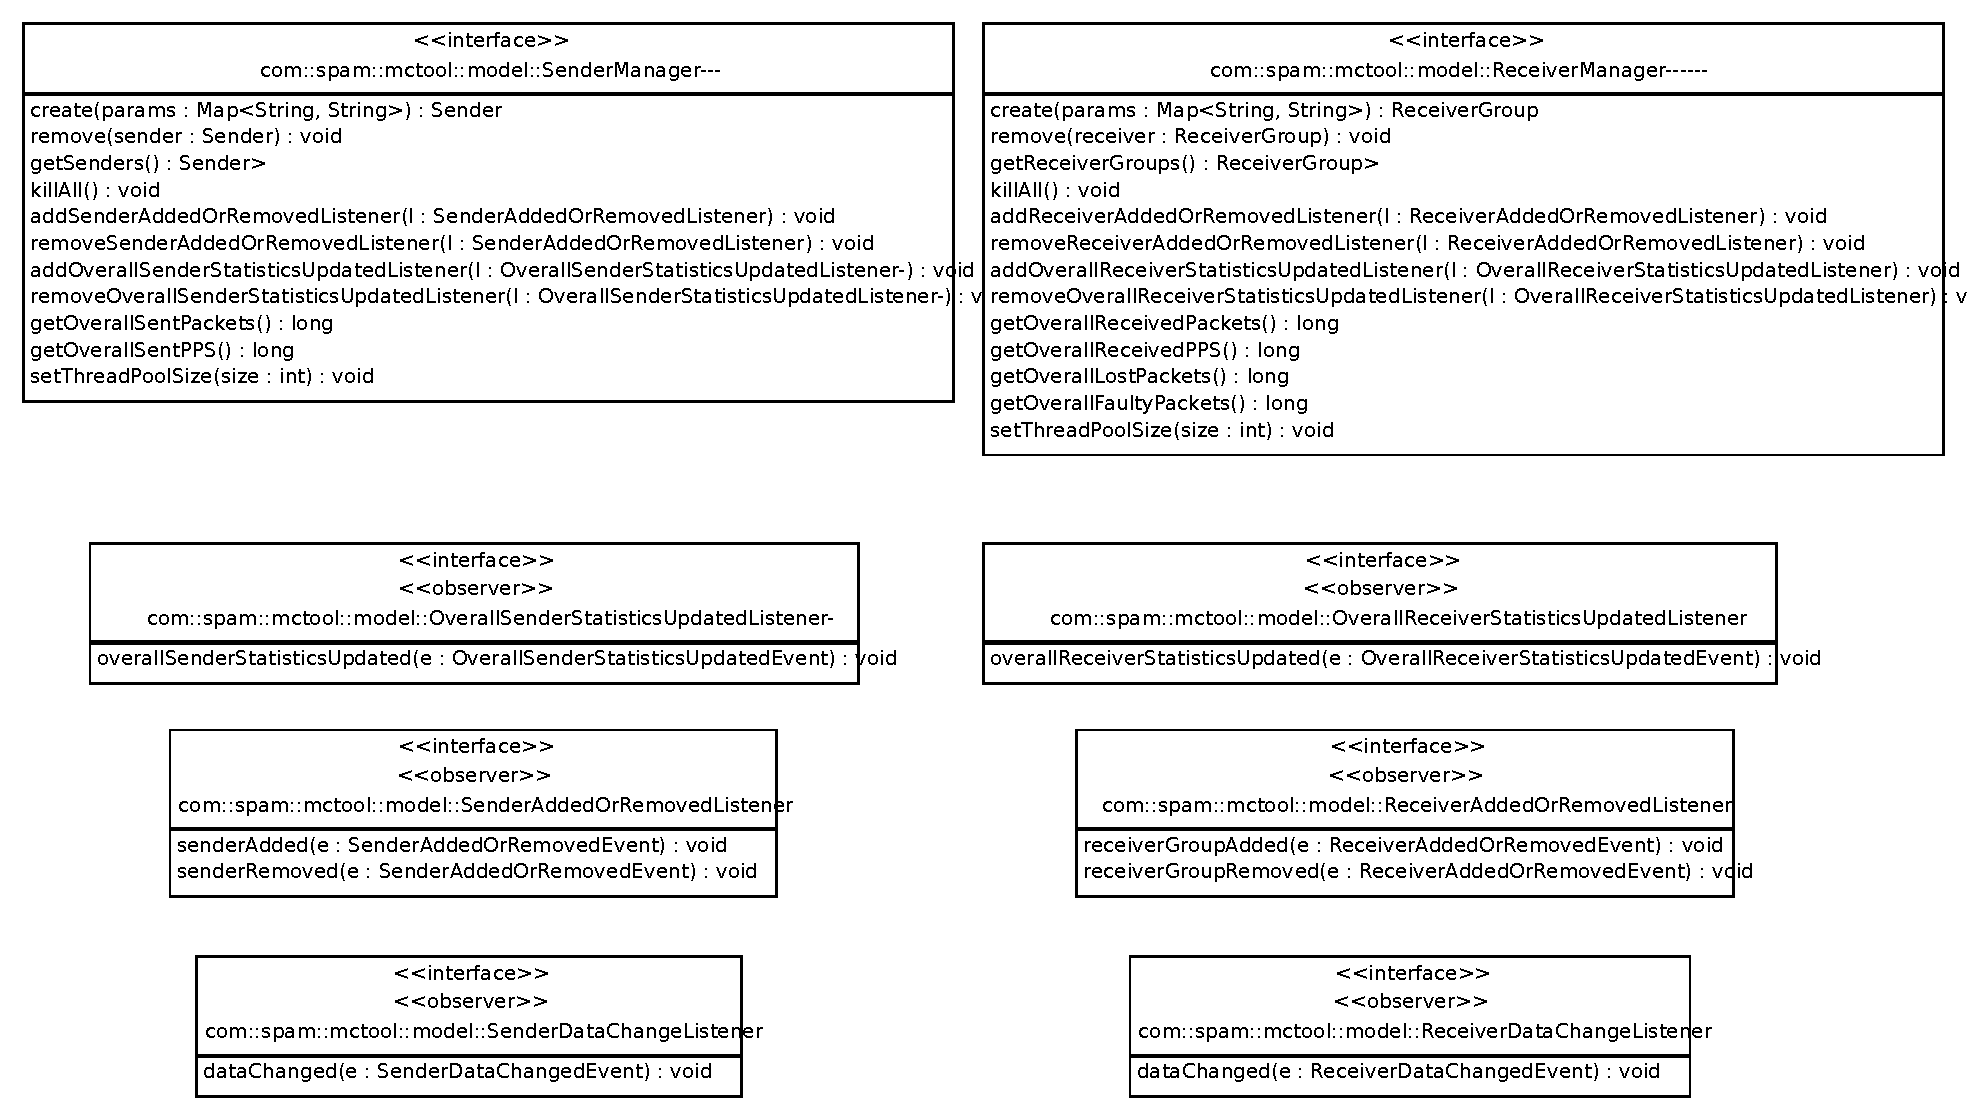
\includegraphics[width=22cm,angle=90]{images/interfaces.pdf}
\caption{Schnittstellen des Modells}
\end{figure}
	

	\end{appendix}

	% Literaturverzeichnis
	%\nocite*{}
	%\bibliographystyle{gerplain}
	%\bibliography{literatur}
	%%%%%%%%%%%%%%%%%%%%%%%%%%%%%%%%%%%%%%%%%%%%%%%%%%%%%%%%%%%%%%%%%%%%%%%%%%%%%%%%

% Dokumentende
\end{document}
